\documentclass[border=12pt]{standalone}
\usepackage{tikz}
\usetikzlibrary{arrows.meta, positioning, calc, fit, backgrounds}
\usepackage{amsmath, amssymb}

\begin{document}
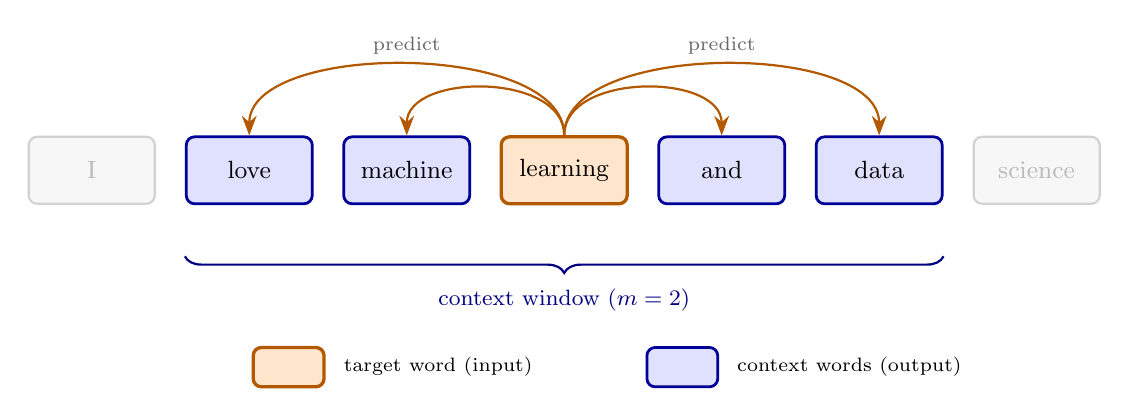
\begin{tikzpicture}[
    word/.style = {rectangle, draw=gray!50, thick, rounded corners=3pt,
                   minimum height=0.85cm, minimum width=1.6cm,
                   font=\small, inner sep=4pt},
    target/.style = {word, draw=orange!70!black, fill=orange!20, line width=1.2pt},
    context/.style = {word, draw=blue!60!black, fill=blue!12, line width=1.0pt},
    outside/.style = {word, fill=gray!6, draw=gray!35, text=gray!55},
    arr/.style = {-{Stealth[length=2.5mm]}, thick, orange!70!black},
    brace/.style = {decorate, decoration={brace, amplitude=6pt, mirror}, thick, blue!50!black},
]

%% ---- Sentence words ----
\node[outside]  (w1) at (0, 0)    {I};
\node[context]  (w2) at (2, 0)    {love};
\node[context]  (w3) at (4, 0)    {machine};
\node[target]   (w4) at (6, 0)    {learning};
\node[context]  (w5) at (8, 0)    {and};
\node[context]  (w6) at (10, 0)   {data};
\node[outside]  (w7) at (12, 0)   {science};

%% ---- Window brace ----
\draw[brace] ([yshift=-0.65cm]w2.south west) -- ([yshift=-0.65cm]w6.south east)
    node[midway, below=8pt, font=\footnotesize, blue!50!black] {context window ($m = 2$)};

%% ---- Prediction arrows from target to context ----
\draw[arr] (w4.north) .. controls +(0, 1.2) and +(0, 1.2) .. (w2.north)
    node[midway, above, font=\scriptsize, black!60] {predict};
\draw[arr] (w4.north) .. controls +(0, 0.8) and +(0, 0.8) .. (w3.north);
\draw[arr] (w4.north) .. controls +(0, 0.8) and +(0, 0.8) .. (w5.north);
\draw[arr] (w4.north) .. controls +(0, 1.2) and +(0, 1.2) .. (w6.north)
    node[midway, above, font=\scriptsize, black!60] {predict};

%% ---- Legend ----
\node[target, minimum width=0.9cm, minimum height=0.5cm, font=\scriptsize]
    (leg1) at (2.5, -2.5) {};
\node[font=\scriptsize, right=3pt of leg1] {target word (input)};

\node[context, minimum width=0.9cm, minimum height=0.5cm, font=\scriptsize]
    (leg2) at (7.5, -2.5) {};
\node[font=\scriptsize, right=3pt of leg2] {context words (output)};

\end{tikzpicture}
\end{document}
